% task1.tex

% Section Title
\section{TASK 1: FREQUENCY-BASED BASELINE} \label{sec:task1}

This section establishes a baseline for malware classification using a frequency-based representation of API call sequences. The intent is to quantify how far one can go with a simple model that ignores temporal order, and to provide a reference point for the more expressive architectures introduced later.

% ------------------------------------------------------------------------------
\subsection{Data Loading and Exploration} \label{subsec:task1_data}

The dataset is provided in JSON format, with each sample containing two fields: \cooltext{api\_call\_sequence} (a list of API function names observed during execution) and \cooltext{is\_malware} (a binary label). Both training and test partitions are loaded for an initial inspection of size, label distribution, and vocabulary.

The training set contains 16,325 samples, while the test set comprises 6,505 samples. A striking observation emerges from examining the class distribution: malware samples constitute 96.26\% of both partitions (15,714 training and 6,262 test samples), leaving only 3.74\% for benign software (611 training and 243 test samples). This severe class imbalance has important implications for model evaluation. Accuracy alone would be misleading, as a trivial classifier predicting ``malware'' for every sample would achieve 96\% accuracy without learning anything meaningful. We therefore pay close attention to precision, recall, and F1-score for both classes, particularly monitoring performance on the minority benign class.

% ------------------------------------------------------------------------------
\subsection{Vocabulary Extraction and Analysis} \label{subsec:task1_vocab}

The frequency-based representation requires a fixed vocabulary. To avoid any information leakage, the vocabulary is extracted from the training set and used to define the feature space at inference time. The training set contains 258 unique API calls, while the test set contains 232.

This immediately exposes a vocabulary mismatch. Twenty-nine API calls appear only in the training set (they can influence training but never occur at test time), while three appear exclusively in the test set: \cooltext{NtDeleteKey}, \cooltext{ControlService}, and \cooltext{WSASocketA}. The latter case is the critical one, because the classifier would be asked to process signals that were not available during training.

Unseen API calls can be handled by introducing an explicit unknown feature (e.g., \cooltext{<UNK>}) or by discarding them when building the input vector. Since the three unseen calls appear in only three test samples, they have negligible impact at the dataset scale; the pipeline therefore ignores them and builds test vectors strictly over the training vocabulary.

% ------------------------------------------------------------------------------
\subsection{Frequency-Based Feature Vectors} \label{subsec:task1_features}

Each API call sequence is transformed into a 258-dimensional vector, where each element is the count of occurrences of a specific API call from the training vocabulary. This bag-of-words representation discards temporal ordering: any permutation of the same multiset of calls maps to the same vector, and patterns that depend on call order are not represented.

The resulting feature matrices are highly sparse, as individual execution traces invoke only a small subset of the full API vocabulary. On average, training samples contain 21.95 non-zero elements per row, representing just 8.51\% of the 258 dimensions. Test samples show slightly higher density with 24.28 non-zero elements (10.46\%). This sparsity has practical implications: memory-efficient sparse matrix representations can be leveraged, and classifiers designed for high-dimensional sparse data become particularly suitable choices.

% ------------------------------------------------------------------------------
\subsection{Classifier Selection and Training} \label{subsec:task1_classifier}

Logistic regression is adopted as the baseline classifier for its computational efficiency on sparse high-dimensional inputs and its transparency: the learned coefficients provide a direct indication of which API calls are associated with either class. The \cooltext{liblinear} solver is selected for its robustness in this regime, while hyperparameters are left at default values to preserve the role of this model as a minimal, reproducible baseline.

A baseline is not a formality. It anchors the comparison with the more complex architectures in the following tasks and prevents attributing improvements to architectural sophistication when the same gains could be achieved by a simpler representation or by exploiting label imbalance.

The data is split into 60\% training and 40\% validation using stratified sampling to preserve class proportions. Training produces a log-loss of 0.0806 on the training set and 0.1225 on the validation set. The gap between these values suggests mild overfitting, but remains acceptable for a baseline model without regularization tuning.

% ------------------------------------------------------------------------------
\subsection{Evaluation and Results} \label{subsec:task1_results}

We evaluate the trained classifier on both validation and held-out test sets. Table~\ref{tab:task1_results} presents the full classification report for the test set.

\begin{table}[h]
\centering
\caption{Frequency-based baseline: classification report (test set)}
\label{tab:task1_results}
\begin{tabular}{lcccc}
\toprule
\textbf{Class} & \textbf{Precision} & \textbf{Recall} & \textbf{F1-Score} & \textbf{Support} \\
\midrule
Benign (0) & 0.6885 & 0.3457 & 0.4603 & 243 \\
Malware (1) & 0.9751 & 0.9939 & 0.9844 & 6,262 \\
\midrule
\textbf{Accuracy} & \multicolumn{3}{c}{0.9697} & 6,505 \\
\textbf{Macro avg} & 0.8318 & 0.6698 & 0.7223 & 6,505 \\
\textbf{Weighted avg} & 0.9644 & 0.9697 & 0.9648 & 6,505 \\
\bottomrule
\end{tabular}
\end{table}

\begin{figure}[H]
            \centering
            \begin{subfigure}[b]{0.48\linewidth}
                \centering
                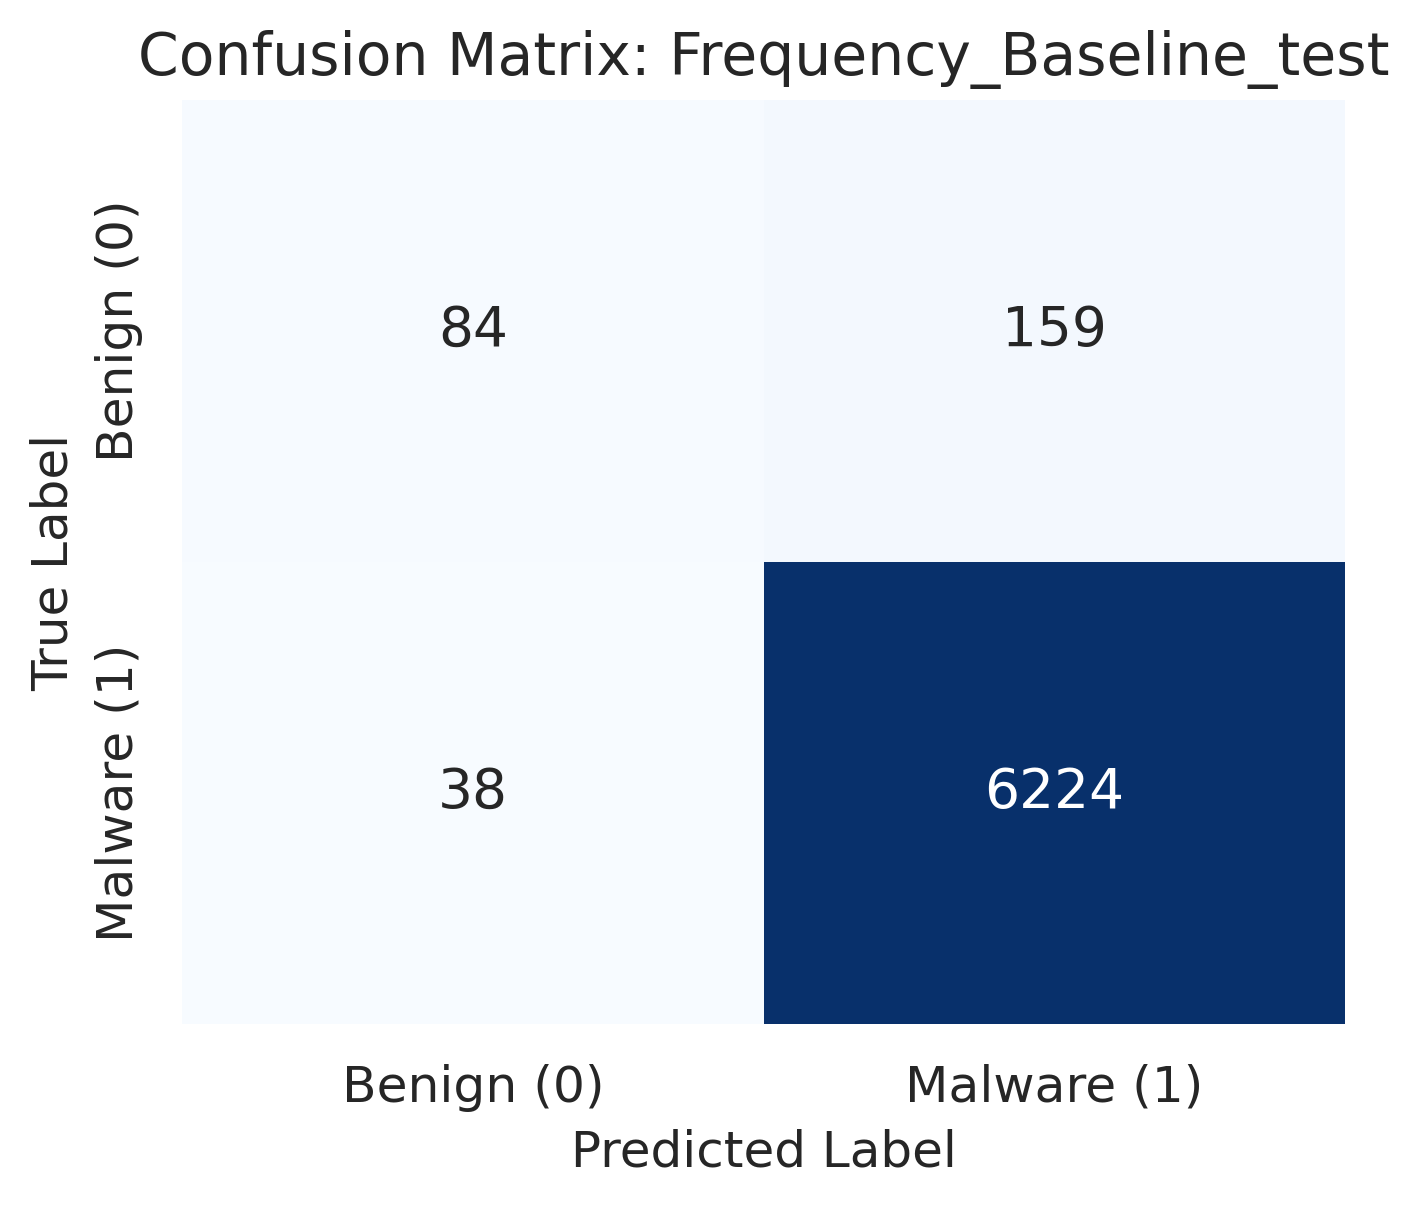
\includegraphics[width=0.9\linewidth]{images/Task1/cm_frequency_baseline_test.png}
                \caption{Confusion matrix for the frequency-based baseline on the test set.}
                \label{fig:task1_cm_test}
            \end{subfigure}
            \hfill
            \begin{subfigure}[b]{0.48\linewidth}
                \centering
                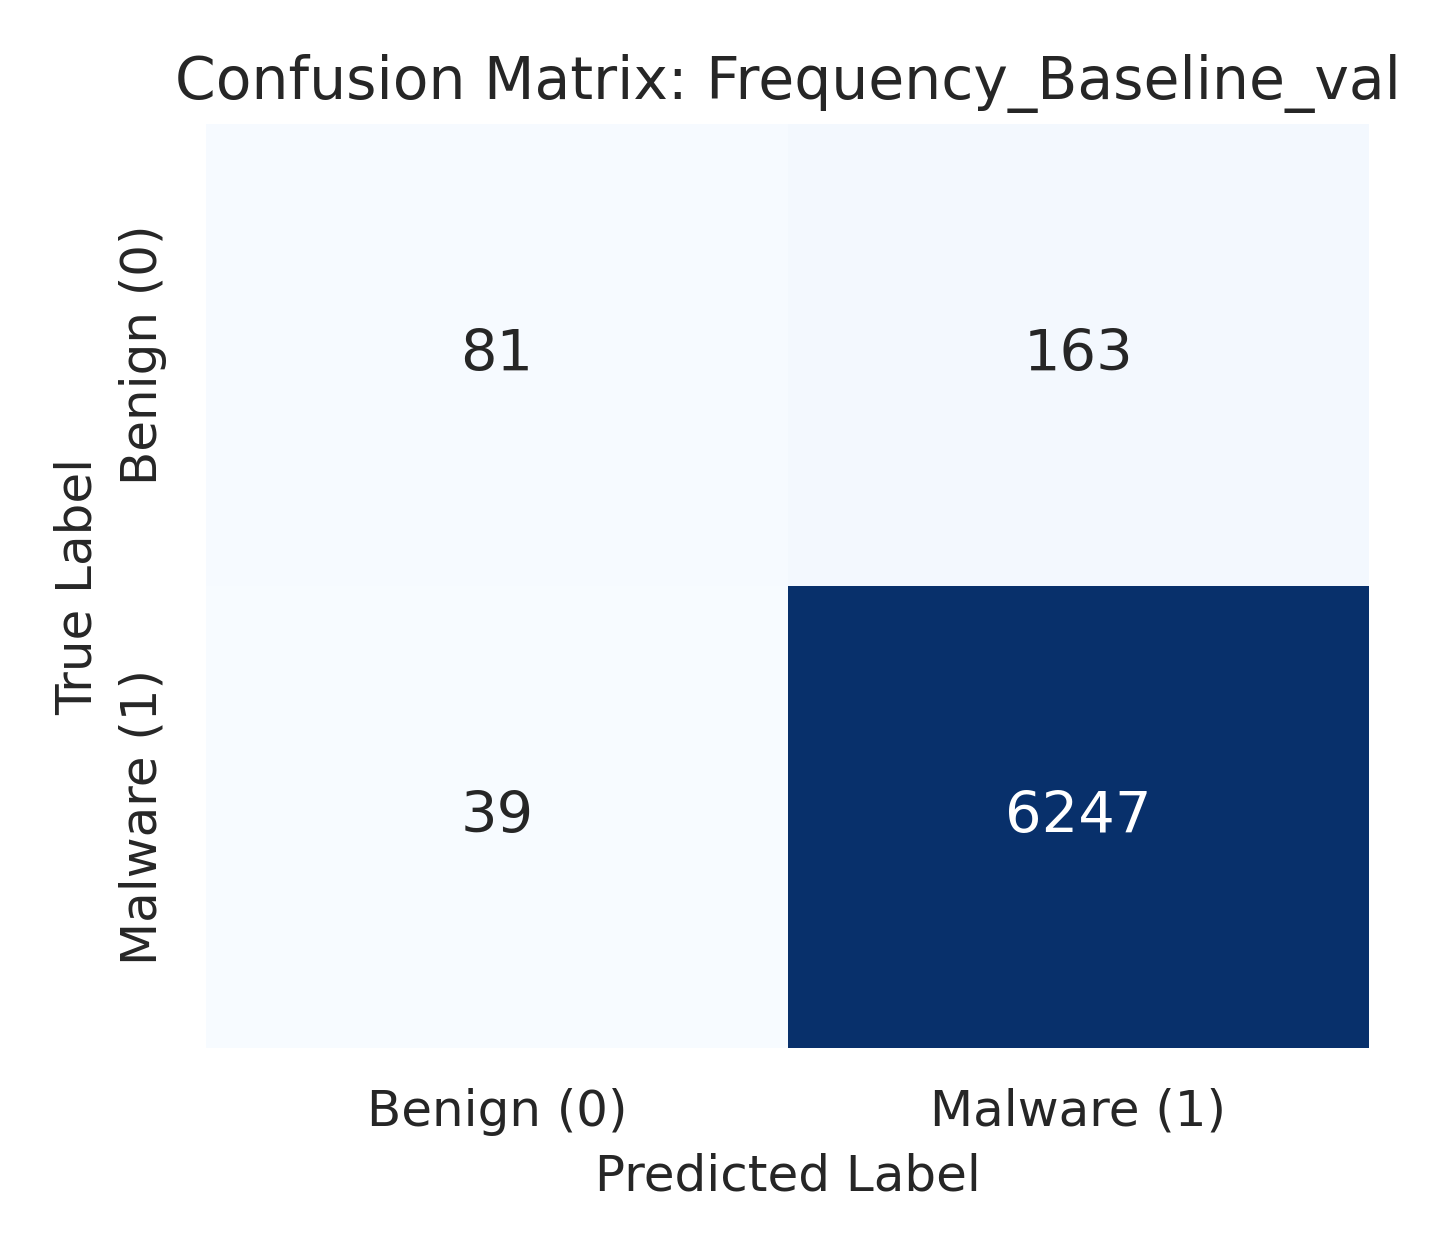
\includegraphics[width=0.9\linewidth]{images/Task1/cm_frequency_baseline_val.png}
                \caption{Confusion matrix for the frequency-based baseline on the validation set.}
                \label{fig:task1_cm_val}
            \end{subfigure}
            \vspace{-0.2cm}
            \caption{Comparison of confusion matrices for the frequency-based baseline on test and validation sets.}
            \label{fig:task1_cm_comparison}
        \end{figure}


The results reveal a markedly asymmetric behavior driven by the underlying imbalance. Malware detection is extremely strong (precision 97.51\%, recall 99.39\%, F1-score 0.9844), and the confusion matrices in Figure~\ref{fig:task1_cm_comparison} confirm that false negatives are rare. The benign class is more challenging: although benign predictions are often correct (precision 68.85\%), recall is low (34.57\%), meaning that a large fraction of benign samples are flagged as malware. With only 3.74\% benign samples, the model learns a conservative decision boundary that favors catching malware at the cost of additional false alarms.

Despite ignoring order and operating on sparse vectors, the frequency-based baseline reaches 96.97\% accuracy and near-perfect malware recall. This shows that the presence and relative frequency of specific API calls already carries substantial discriminative signal, even before exploiting sequential dependencies.

The limitation is structural: frequency vectors cannot represent temporal motifs, repeated call patterns, or long-range dependencies. This motivates the sequence- and structure-aware models in the subsequent tasks, where the representation is designed to preserve more of the behavioral dynamics that are erased by the bag-of-words transformation.